\chapter{Particle Interaction Theory}
\label{chap:particle-interaction-theory}

This chapter will give a brief introduction to the theory of systems of pairwise-interacting particles, to pave the way for the upcoming discussion of numerical methods for the solution of their density distribution function.
% particle simulations as well as a spectral method

\section{A Many-Body System}
An $N_p$-body system is a discrete set of particles with associated position $\vec{x_i} \in \R^d$ and velocity $\vec{v_i} := \frac{\dd\vec{x_i}}{\ddt} \in \R^d$ interacting with one another.
Each particle individually is subject to inertia and its kinetic energy (``second moment'' \footnote{
  In kinetic theory, the $0$th moment is the mass $m_i$ of a particle, the first moment is the momentum $\vec{\hat{p}_i}$ and the second moment is its kinetic energy $E_{kin,i}$.
}) is given by
$$E_{\text{kin},i} = \frac{\vec{\hat{p}_i}^2}{2m} = \frac{(m \vec{\hat{v}_i})^2}{2m} = \frac{1}{2} m \norm{\vec{\hat{v}_i}}^2\,.$$
The second important ingredient is an interaction potential motivating pairwise forces $\vec{F_{ij}} \in \R^d$ between particles
$$\vec{F_{ij}} = -\nabla U_{ij} = -\left(\partial x_1, ..., \partial x_d\right)^T U_{ij}\,.$$

The total potential of a system of $N_p \ge 2$ particles $U \in \R$ can be calculated by summing up the pair potentials $U_{ij} \in \R$ between all pairs of particles
$$U = \sum_{i=1}^{N_p}\sum_{j=1, j \neq i}^{N_p} U_{ij} = \sum_{i=1}^{N_p}\sum_{j=1, j \neq i}^{N_p} K\left(\norm{\vec{\hat{x}_i} - \vec{\hat{x}_j}}\right)\,,$$
where $\vec{\hat{x}_i} \in \R^d$ represents the $d$-dimensional position of particle $i$, respectively.

In the absence of an external potential $V$, the total energy of the particle system is given by $E = E_{\text{kin}} + U$, so
\begin{equation}
  E = \frac{1}{2} \sum_{i=1}^{N_p} m_i \vec{\hat{v}_i}^2 + \sum_{i=1}^{N_p}\sum_{j=1, j \neq i}^{N_p} K\left(\norm{\vec{\hat{x}_i} - \vec{\hat{x}_j}}\right)\,.
  \label{eq:total-energy}
\end{equation}

Following from Newton's equations of motion together with a model for friction and self-propulsion (cf. \Cref{sec:self-propulsion-friction}), each particle $i=1, ..., N_p$ at position $\vec{\hat{x}_i} \in \R^d$ and time $t \in \R^+$ then follows
\begin{equation}
  \frac{\dd^2 \vec{\hat{x}_i}}{\ddt^2} = f\left(\norm{\frac{\dd \vec{\hat{x}_i}}{\ddt}}\right) \frac{\dd\vec{\hat{x}_i}}{\ddt} - \frac{1}{N} \sum_{j=1, i\neq j}^{N} \nabla K\left(\norm{\vec{\hat{x}_i} - \vec{\hat{x}_j}}\right)\,,
  \label{eq:evolution-equation}
\end{equation}
for reference see, for example, \cite{2020-power-law-kernels, 2021-arbitrary-dimensions, 2017-explicit-solutions}.
For now, we only consider the case without an external potential $V(\hatvec{x})$.

\section{Continuous Limit}
The evolution equation \eqref{eq:evolution-equation} without friction or self-propulsion, in the mean-field limit as $N_p \goesto \infty$, becomes
\begin{equation}
  \frac{\partial \hat{\rho}}{\partial t} = \nabla \cdot \left(\hat{\rho} \nabla K * \hat{\rho}\right)\,.
  \label{eq:continuous-evolution-equation}
\end{equation}
where $\hat{\rho}: \R \to \R$ is the particle density function and $*$ denotes a convolution.
More details are given in \cite{2014-carrillo-derivation-of-mean-field, 2021-carrillo-radial}.
The solution $\hat{\rho}$ we are looking for within the scope of this dissertation is the \textit{equilibrium measure} (cf. \Cref{def:equilibrium-measure}), a particle density distribution function minimising the total potential $U$.

\begin{definition}{Equilibrium Measure}{equilibrium-measure}
  For a given pairwise interaction potential $K: \R \to \R$, the equilibrium measure $\hat{\rho}: D \to \R$ with $D \subseteq \R^d$ is a measure chosen such that
  $$U_K[\hat{\rho}] := \frac{1}{2} \iint K\left(\norm{\hatvec{x} - \hatvec{y}}\right) \,\dd\hat{\rho}(\hatvec{x})\,\dd\hat{\rho}(\hatvec{y})\,,$$
  is minimised, where $\dd\hat{\rho} = \hat{\rho}(\hatvec{x})\dd\hatvec{x}$.
\end{definition}
Also consider the total mass of the equilibrium distribution, given by
\begin{equation}
  M[\hat{\rho}] := \int \dd\hat{\rho} = \int_{\supp(\hat{\rho})} \hat{\rho}(\hatvec{x}) \,\dd\hatvec{x}\,,
  \label{eq:measure-mass}
\end{equation}
which, without loss of generality, we can choose to equal $1$ to make $\hat{\rho}(\hatvec{x})$ a \textit{probability distribution}, which provides a useful interpretation of values of $\hat{\rho}$:
The probability of finding a particle in a volume $\mathcal{V} \subseteq B_R(\vec{0})$ is given by $\int_{\mathcal{V}} \hat{\rho}(\vec{x}) \,\dd\vec{x}$.
Also note that, as the integrand of the above integrals, we sometimes refer to the interaction potential $K(r)$ as an integral kernel or simply \textit{kernel}.

Due to the absence of an external potential, solutions are translationally invariant, so for simplicity we can choose them to be centred at the origin.
That is, on $D = B_R(\vec{0})$ instead of $B_R(\hatvec{x}_{\text{centre}})$, where $\vec{x}_{\text{centre}} := \frac{1}{N_p} \sum_{i=1}^{N_p} \vec{x_i}$ with $R \in \R^+$ usually chosen as the smallest possible $R$ such that $\supp(\rho) \subseteq [-R, R]$.

As throughout the rest of this document, we restrict ourselves to radially symmetric solutions, we will use $\hatvec{x} := R\hatvec{x} \in B_R(\vec{0})$ to denote position in the original $d$-dimensional ball domain of radius $R$, whereas $\vec{x} \in B_1(\vec{0})$ denotes position in the normalised domain with radius $1$.
Solutions on the original domain shall be denoted by $\hat{\rho} \in \functionspacehat$ whereas equilibrium measures $\rho \in \functionspace$ denote solutions on the normalised domain $B_1(\vec{0})$ with $\functionspace$ and $\functionspacehat$ given in \Cref{def:function-space}.
Therefore, $\supp(\hat{\rho}) = B_1(\vec{0})$ and $\supp(\rho) = B_R(\vec{0})$.
The relationship between them is simply, $\hat{\rho}(\hatvec{x}) = \hat{\rho}(R\vec{x}) = \rho(\vec{x})$.

\begin{definition}{Space of Particle Density Distributions}{function-space}
  On the \textit{full domain} $B_R(\vec{0}) \subset \R^d$, let
  $\functionspacehat := \{\rho: B_R(\vec{0}) \to \R\}\,.$
  On the \textit{normalised domain} $B_1(\vec{0})$ of radius $1$, let
  $\functionspace := \{\rho: B_1(\vec{0}) \to \R\}\,.$
\end{definition}

For a given density distribution $\rho$, we define a utility operator to help with notation, the power law potential (\Cref{def:power-law-potential}).

\begin{definition}{Power Law Potential Energy}{power-law-potential}
  For a given equilibrium measure $\rho \in \functionspace$ and $\beta \in \R$, the power law potential operator $U_K: \functionspace \to \R$ is given by
  $$U^{(\beta)}[\rho] := \iint \norm{\vec{x}-\vec{y}}^\beta \,\dd\rho(\vec{x})\dd\rho(\vec{y})\,.$$
\end{definition}

Note that because
$$\iint \norm{\vec{x}-\vec{y}}^\beta \,\dd\rho(\vec{x})\dd\rho(\vec{y}) = \iint_{\supp(\rho)^2} \norm{\vec{x}-\vec{y}}^\beta \rho(\vec{x}) \rho(\vec{y}) \,\dd\vec{x}\dd\vec{y}\,,$$
\Cref{def:power-law-potential} also generalises to $\hat{\rho} \in \functionspacehat$ thanks to the definition as a measure, and after a change of variables from $\vec{x}$ to $\hatvec{x}$ and $\vec{y}$ to $\hatvec{y}$, we obtain the relationship
$$U^{(\beta)}[\hat{\rho}] = R^{2d + \beta} U^{(\beta)}[\rho]\,.$$

With these preliminaries in mind, we can now formulate \href{def:the-problem}{the problem}.

\begin{definition}[colframe=gray, colbacktitle=gray!30]{Particle Density Distribution Problem}{the-problem}
  Given an interaction kernel $K: \R^+ \to \R$, the density distribution problem is to find the equilibrium measure $\hat{\rho}: B_R(\vec{0}) \to \R$ of mass $M = 1$ on a $d$-dimensional ball of radius $R \in \R^+$ that minimises the total potential $U_K[\hat{\rho}]$.
\end{definition}

\section{Interaction Potentials}
We present a brief overview of the interaction potentials considered within the scope of this dissertation.

\subsection{Attractive-Repulsive Potential}
One example we study is that of the attractive-repulsive interaction potential, where two power law potentials compete with each other.
For a given $\alpha, \beta \in \R \backslash \{0\}$, it is given by
\begin{equation}
  K_{\alpha, \beta}(r) = \frac{r^\alpha}{\alpha} - \frac{r^\beta}{\beta}\,.
  \label{eq:attractive-repulsive-potential}
\end{equation}
One can even consider the case when either $\alpha$ or $\beta$ is 0 in order to arrive at a log-term \parencite{2017-explicit-solutions}, using $\frac{x^0}{0} := \log(x)$ as a convention\footnote{
  Consider the Laurent series expansion of $\frac{x^a}{a} = \frac{1}{a} + \log(x) + \frac{1}{2}a \log^2(x) + \mathcal{O}(a^2)$ in the limit as $a \goesto 0^+$.
  While this limit approaches $\infty$ coming from the right and $-\infty$ coming from the left due to the nature of the first term in the expansion, the only remaining term in it is $\log(x)$ which is thereby chosen as a convention.
}.
If the repulsive term is stronger (i.e. $\beta > \alpha$), there is no equilibrium distribution as particles simply continue repelling each other out to infinity.
Attractive-repulsive potentials in general describe pairwise interactions with separate attractive and repulsive terms.
In our case however, we will only refer to attractive-repulsive \textit{power law} potentials, specifically of the form in \Cref{eq:attractive-repulsive-potential}.
Its equilibrium distance is at $r = 1$.

% Some input from the Wolfson Particle Physicist
The Lennard-Jones potential ($\alpha=-12, \beta=-6$), for example, is an \textbf{intermolecular} potential, so the relevant length-scale is between molecules.
Therefore, the only relevant interaction is the electromagnetic force.
Other forces, such as the strong force which keeps protons in the nucleus together (a force much stronger than the electromagnetic one, but effective only at much smaller distances), need not be considered at this length-scale.

\subsection{Morse Potential}
Another frequently used pairwise interaction is the \textit{Morse potential} $K_{C_a, l_a, C_r, l_r}: \R^+ \to \R$ given by
\begin{equation}
  K_{C_a, l_a, C_r, l_r}(r) := C_a \e^{-r / l_a} - C_r \e^{-r / l_r}\,,
  \label{eq:morse-potential}
\end{equation}
with attractive parameters $C_a \in \R^+$ and $l_a \in \R^+$ (a `natural length scale') and repulsive parameters $C_r, l_b \in \R^+$.
Possible parameter ranges are given by $C_a l_a^{d-2} > 1, l_a < 1$ \parencite{2006-self-propelled,2014-explicit-flock-solutions-for-quasi-morse-potentials}.

\subsection{Mixed Potential}
Combining the above approaches of power law and exponential decay interaction potentials, we can define
\begin{equation}
  K_{(C, l, \bar{a})}(r) := \frac{r^{\bar{a}}}{\bar{a}} + C e^{-r/l}\,,
  \label{eq:mixed-potential}
\end{equation}
the combination of both.
Its solution via spectral methods, as introduced later in \Cref{chap:spectral-method,chap:general-kernel-spectral-method}, can be constructed in an efficient manner exploiting the structure of the potential together with the general kernel ansatz.

\subsection{Absolute Value Potential}
As part of an exploration of the various types of kernels, one can consider
\begin{equation}
  K_{||}(r) := |1-r|\,,
  \label{eq:absvalue-potential}
\end{equation}
as depicted in \Cref{fig:comparing-potentials}.
Its equilibrium distance is at $r = 1$.
Because the function is not continuously differentiable, this potential is entirely un-physical but yields interesting results nonetheless (cf. \Cref{fig:gyroscope-quiver-3d}).

\begin{figure}[H]
  \centering
  \inputtikz{comparing-potentials}
  \caption[Comparing potentials]{Comparing Potentials: The attractive-repulsive potential $K_{(\alpha,\beta)}(r)$ with $(\alpha,\beta) = (3.5, 1.6)$, the Morse potential $K_{(C_a, l_a, C_r, l_r)}(r)$ with $(C_a, l_a, C_r, l_r) = (1.5, 2.0, 1.0, 0.5)$, the mixed potential $K_{C, l, \bar{a}}$ with $(C, l, \bar{a}) = (1.0, 0.5, 1.8)$ and the absolute value potential $K_{||}(r)$.}
  \label{fig:comparing-potentials}
\end{figure}

The remaining chapter will briefly discuss analytical approaches taken in particle physics and computational biology to solve a version of the above problem given in \Cref{def:the-problem}.

\section{Self-Propulsion and Friction}
\label{sec:self-propulsion-friction}
In order to model animals in a swarm, it makes sense to consider the effect of self-propulsion (a force accelerating the particle in the direction it is already going).
A set of particles with this ability are referred to as active matter - a number of individual agents within a medium.
Friction is the opposite of that - a force acting against movement, cf. \Cref{eq:evolution-equation}.
Self-propulsion and friction could be modelled as a quadratic of the form
$$f(\hat{v}_i) = f_{\rm self-propulsion} - f_{\rm } \hat{v}_i^2\,,$$
with $\hat{v}_i := \norm{\vec{\hat{v}_i}} = \norm{\frac{\dd\vec{\hat{x}_i}}{\ddt}}$ the absolute value of the velocity of particle $i$.
Running a simulation using the Morse potential given in \Cref{eq:morse-potential} with this friction model results in a good archetype for animal swarming behaviour, as seen in \Cref{fig:simulation-quiver-illustration}.
This approach is taken from \cite{2006-self-propelled} and we are able to reproduce their simulation results.

\begin{figure}[H]
  \centering
  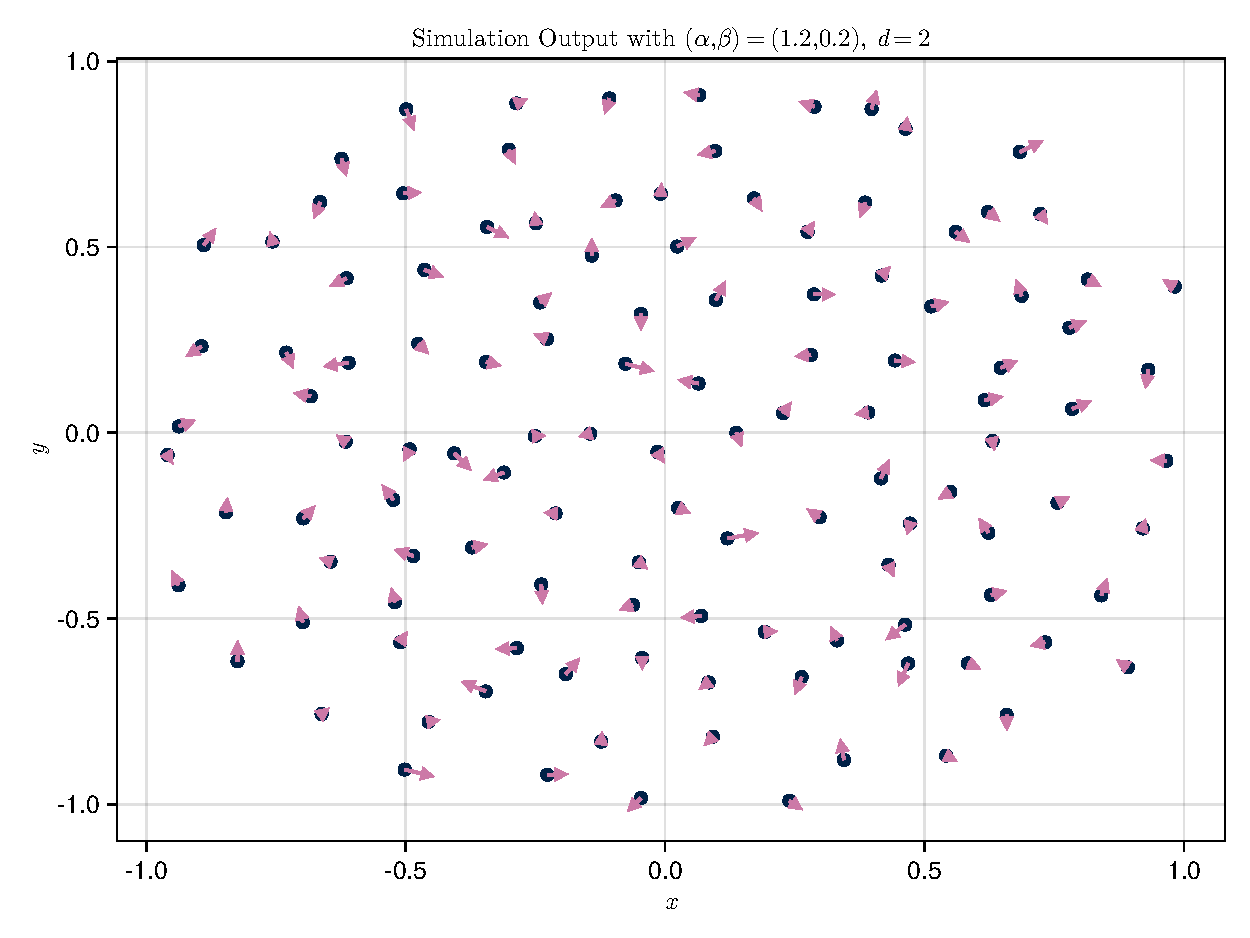
\includegraphics[width=0.8\linewidth]{results/morse-2d/simulation-quiver.pdf}
  \caption[Quiver plot of 120 particles in 2D interacting through the Morse potential]{Position and velocity of $N_p = 120$ particles $d = 2$ dimensions as obtained through the molecular dynamics simulation introduced in \Cref{chap:particle-simulator}. The interaction potential is a Morse potential with given parameters. Friction and self-propulsion terms are present as described in \cite{2006-self-propelled}, so using $f(v_i) = 1.6 - 0.5 v_i^2$, this figure reproduces their results.}
  \label{fig:simulation-quiver-illustration}
\end{figure}

\section{Kinetic Theory: The Vlasov Equation}
A common tool in plasma physics is the Vlasov equation,
$$\frac{\partial f}{\partial t}+{\frac {\dd \vec{r} }{\dd t}}\cdot {\frac {\partial f}{\partial \vec{r} }}+{\frac {\dd \vec{p} }{\dd t}}\cdot {\frac {\partial f}{\partial \vec{p} }}=0\,,$$
describing the change of the phase-space distribution function $f(\vec{r}, \vec{p}, t)$ over time.
The Vlasov equation is the collisionless Boltzmann equation, Vlasov replaces the collision term with long-range interactions.

An important result in kinetic theory is Liouville's theorem, stating that the total volume occupied in phase-space $\R^{2dN_p}$ of $d$ coordinates for position and velocity for $N_p$ particles is constant.

\begin{theorem}{Liouville's Theorem}{liouville}
  Phase-space volume is conserved in situations of pure particle-particle interactions
  $$\frac{\dd f}{\ddt}=
    \frac{\partial f}{\partial t}
    +\sum_{i=1}^n\left(\frac{\partial f}{\partial q_i}\dot{q}_i
    +\frac{\partial f}{\partial p_i}\dot{p}_i\right)=0\,.$$
\end{theorem}

This observation can be used to verify, for instance, the correctness of large molecular dynamics simulations.

\section{Swarming in Biological Settings}
A 2010 paper by \citeauthor{2010-starlings} showed the surprising result that correlation between movement of individual starlings in bird flocks over Rome is scale-free.
In contrast to the assumption that birds only mirror their neighbours' behaviour and swarming behaviour emerges as a result of that, this observation suggests that bird flocks exert collective behaviour beyond local interactions.
\begin{quote}
  ``\textit{The change in the behavioural state of one animal affects and is affected by that of all other animals in the group, no matter how large the group is}.'' - \cite{2010-starlings}.
\end{quote}
Their study was carried out by individually tracking each starling in the flock and using tracking algorithms to represent their 3 dimensional positions and velocities.

\subsection{Vicsek Model}
The Vicsek model \parencite{1995-vicsek-model} is intended for the study of active matter, in particular it is suitable to describe the swarming behaviour of large groups of animals.
The fundamental idea behind the model is to assume local alignment of velocities $\vec{v_i}$ within a swarm of animals, suggesting that birds or fish imitate the direction of their neighbours.
It describes how large-scale, collective motion emerges from small-scale, local interactions.

\subsection{Long-Range Interaction Potentials}
The approach we will take within the scope of this dissertation is to model animal swarms as a continuum and introduce long-range interactions where each particle not only interacts with its closest neighbours but also far-away particles, as suggested empirically in \cite{2010-starlings}.

\section{Analytical Solutions}
\label{sec:analytical-solutions}
\cite{2017-explicit-solutions} provides some analytical, radially symmetric solutions to \hyperref[def:the-problem]{the problem}, local minima of the energy.
More recently, \cite{2021-carrillo-radial} could show that the solution is indeed a global minimiser of the total energy.
For example, with an attractive-repulsive potential as given in \Cref{eq:attractive-repulsive-potential}, when $\alpha = 2$ and $\beta \in [-1, 2]$, the equilibrium measure is given by
\begin{equation}
  \hat{\rho}(\hatvec{x}) = C_\beta \cdot R^d \cdot \left(R^2 - \hatvec{x}^2\right)^{\frac{1-\beta}{2}}\,,
  \label{eq:analytical-solution-alpha-equal-2}
\end{equation}
where
$$C_\beta := \frac{1}{(\beta - 1) \pi} \cos\left(\frac{(2 - \beta) \pi}{2}\right)\,,$$
$$R := \left(C_\beta \cdot B\left(\frac{1}{2}, \frac{3 - \beta}{2}\right)\right)^{\frac{1}{\beta - 2}}\,,$$
with $B(\cdot, \cdot)$ the beta-function (cf. \Cref{def:beta-function}).
